
\chapter{2D wings in compressible flow}
\section{Subsonic flows}
\subsection{The Prandtl-Glauert relation}
	Remind that we have defined a potential function to describe incompressible flows, conservation of mass giving:
	
	\begin{equation}
	\vec{v} = \nabla \phi \qquad \frac{\D u}{\D x} + \frac{\D v}{\D y} = 0 = \frac{\D^2 \phi}{\D x^2} + \frac{\D^2 \phi}{\D y^2}.
	\end{equation}
	
	This can also be used to describe compressible flows, conservation of mass is then: 
	
	\begin{equation}
	\rho (\phi _{xx} + \phi _{yy}) + \rho _x \phi _x + \rho _y \phi _y = 0
	\label{eq:6.2}
	\end{equation}
	
	where we introduced the shorthand notation $\frac{\D a}{\D x} = a_x$. We assume that the flow is isentropic, this is satisfied by inviscid flows (no shock  wave): 
	
	\begin{equation}
	\frac{\rho}{T^{\frac{1}{\gamma -1}}} = cst \qquad \Rightarrow \frac{d \rho}{\rho} = \frac{1}{\gamma -1} \frac{dT}{T}
	\end{equation}
	
	if the flow does not work (turbine), the temperature is constant and the equation becomes:
	
	\begin{equation}
	d\rho = -\frac{\rho}{2a^2} d(u^2+v^2).
	\end{equation}

	If we replace the velocities we get: 
	
	\begin{equation}
	\rho _x = -\frac{\rho}{a^2} (\phi _x \phi _{xx} + \phi _y \phi _{xy}) \qquad \rho _y = -\frac{\rho}{a^2} (\phi _x \phi _{xy} + \phi _y \phi _{yy}).
	\end{equation}		
	
	That we can substitute in \eqref{eq:6.2}:
	
	\begin{equation}
	\left( 1-\frac{1}{a^2} \phi^2_x \right) \phi _{xx} + \left( 1-\frac{1}{a^2 }\phi^2_y \right) \phi _{yy} - \frac{2}{a^2} \phi_x \phi_y \phi _{xy} = 0.
	\label{eq:6.6}
	\end{equation}		
	
	We can now apply this to an airfoil, if the far field velocity profile is $u= V_\infty$, we can note the velovity field by means of perturbations: $u = V_\infty + \hat{u}, v = \hat{v}$. A perturbation potential function can be defined: 
	
	\begin{equation}
	\phi = V_\infty x + \hat{\phi}\qquad with \qquad \hat{\phi} _x = \hat{u}, \quad \hat{\phi}_y = \hat{v}. 
	\end{equation}
	
	By substitution of this in \eqref{eq:6.6}:
	
	\begin{equation}
	\left[ a^2- (V_\infty + \hat{\phi} _x )^2 \right] \hat{\phi} _{xx} + \left[ a^2-\hat{\phi}_y ^2 \right] \hat{\phi} _{yy} - 2 (V_\infty + \hat{\phi} _x) \hat{\phi}_y \hat{\phi} _{xy} = 0.
	\label{eq:6.8}
	\end{equation}
	
	Since the total temperature is constant:
	
	\begin{equation}
	\frac{a^2_\infty}{\gamma -1} + \frac{V_\infty ^2}{2} = \frac{a^2}{\gamma -1} + \frac{(V_\infty + \hat{u}) ^2 = \hat{v}^2}{2} 
	\label{eq:6.9}
	\end{equation}
	
	If we make the assumption of small perturbation, the quadratic terms cancel and \eqref{eq:6.8} and \eqref{eq:6.9} become:
	
	\begin{equation}
	\begin{aligned}
	&\frac{a^2_\infty}{a^2} = 1 - (\gamma -1) \frac{\hat{u}}{V_\infty} M^2_\infty\\
	&\left[ a^2- V^2_\infty + 2V_\infty \hat{u}  \right] \hat{\phi} _{xx} + a^2 \hat{\phi} _{yy} - 2 V_\infty \hat{v} \hat{\phi} _{xy} = 0 \\ 
	\Rightarrow 
	&\left[ 1- M_\infty^2 - (\gamma + 1) M_\infty \frac{\hat{u}}{V_\infty} \right] \hat{\phi} _{xx} + \left[ 1 - (\gamma -1 )M_\infty ^2\frac{\hat{u}}{V_\infty} \right] \hat{\phi} _{yy} - 2 M^2_\infty \frac{\hat{v}}{V_\infty} \hat{\phi} _{xy} = 0 
	\end{aligned}
	\end{equation}
	
	where the last expression is obtained by dividing by $a^2_\infty$ and replacing. By considering again the small perturbation ($V_\infty \ll$) equation we get the:
	
	\begin{center}
	\theor{
	\textbf{Transonic smal perturbation potential equation}
	\begin{equation}
	\left[ (1-M_\infty ^2) - (\gamma +1) M^2_\infty \frac{\hat{\phi}_x}{V_\infty}  \right] \hat{\phi} _{xx} + \hat{\phi} _{yy} = 0.
	\end{equation}
	}
	\end{center}
	
	We can see that the $\hat{u}$ appears in $\\hat{phi} _{xx}$ term, this is no longer negligible for \textbf{sonic} velocities. For sub- and super-sonic flows however the equation simplifies in: 
	
	\begin{equation}
	(1-M_\infty ^2) \hat{\phi} _{xx} + \hat{\phi} _{yy} = 0.
	\end{equation}
	
	Note that we retrieve our incompressible equation for $M_\infty \rightarrow 0$. Be aware that this last relation is only valid for small perturbations (small bodies in practice) and sub- or super-sonic flows ($M_\infty > 1.2, M_\infty < 0.8$). \\
	
	Let's now operate a change of coordinate $(x,y) \rightarrow (\xi , \eta)$, recalling $1-M_\infty ^2 \equiv \beta ^2$: 
	
	\begin{equation}
	\xi = x \quad \eta = \beta y \qquad \bar{\phi} (\xi , \eta) = m .\hat{\phi}(x,y)
	\end{equation}
	
	where m is a constant. Let's find the expression of $\bar{\phi} (\xi, \eta)$. The chain rule gives: 
	
	\begin{equation}
	\begin{aligned}
	\hat{\phi} _x = \hat{\phi}_\xi = \frac{1}{m} \bar{\phi} _\xi \qquad  \hat{\phi} _y = \frac{\beta}{m} \bar{\phi}_\eta &\qquad \hat{\phi} _{xx} = \frac{1}{m} \bar{\phi}_{\xi \xi} \qquad \hat{\phi} _{yy} = \frac{\beta ^2}{m} \bar{\phi}_{\eta \eta}\\
	&\Rightarrow \bar{\phi}_{xx} + \bar{\phi}_{yy} = 0
	\end{aligned}
	\label{eq:6.14}
	\end{equation}
	
	We can see that the compressible flow in $(x,y)$ is reduced to an incompressible flow in the $(\xi, \eta)$ plane. Pay attention that $\bar{\phi}$ describes the perturbation velocities $\bar{u}, \bar{v}$. in the $(\xi, \eta)$ plane.  
	
	\wrapfig{7}{l}{7.5}{0.1}{ch6/9}{fig:6.9}
	We can now focus on the shape of the profile in the new axis. Let's analyze the tangent to the profile by defining the angle $\theta$ for the profile in (x,y). Under the assumption of small perturbation (thin airfoil), we can see that:
	
	\begin{equation}
	\tan \theta \approx \theta = \frac{\hat{v}}{V_\infty + \hat{u}} \approx \frac{\hat{v}}{V_\infty} = \frac{1}{V_\infty} \hat{\phi} _y \qquad \Rightarrow \chi \approx \frac{1}{V_\infty} \bar{\phi} _\eta
	\end{equation}
	
	where the analogy for the new plane is done. Using \eqref{eq:6.14}, we get: 
	
	\begin{equation}
	\theta = \frac{\beta}{m} \chi.
	\end{equation}
	
	Let's investigate two cases: 
	\begin{itemize}
	\item[•] If we choose $m=\beta$, $\theta = \chi$, the two profiles are identical. We have for the velocity: 
	
	\begin{equation}
	\hat{u} = \hat{\phi} _x = \frac{\bar{\phi}_\xi}{\beta} = \frac{\bar{u}}{\beta}
	\end{equation}
	
	and since the pressure coefficient is given by $C_p = -\frac{2\hat{u}}{V_\infty}$: 
		\end{itemize}		
		
	\begin{center}
	\theor{
	\textbf{Prandtl-Glauert rule}
	\begin{equation}
	C_p = \frac{C_{p,inc}}{\beta} = \frac{C_{p,inc}}{\sqrt{1 - M_\infty ^2}}.
	\end{equation}
	This equation allows us to compute the pressure distribution in compressible flow, beginning from the incompressible one. 
	}
	\end{center}

	
	\wrapfig{12}{r}{5}{0.15}{ch6/10}{fig:6.10}
	Since the lift and moment coefficient are given by the integration of the pressure coefficient along the wing, we have the same result for them (so also the slope of lift curve $m$). Here is plotted the experimental data and the approximated m by means of the above relation for $\alpha = 0$ and for different airfoil thickness $\tau$. We can see that for the thinner wings, we have a good agreement, until we reach the \textbf{critical Mach number} (Mach number at infinity for which Mach number 1 is reached on the profile).  This value exceeded, we have shock waves (formula valid only for Mach until 0.8). 
	For thicker wings, we see that the slope m is always underestimated. The critical Mach number is here much lower. 
	
	\ \\
\begin{itemize}
	\item[•] If we choose $m=1, \hat{u} = \bar{u}$ so that $C_p = C_{p, inc}$. We see that the pressure coefficient is now the same but the profiles are different following we are in the compressible or incompressible case $\theta = \beta \chi$. 
\end{itemize}

\wrapfig{5}{l}{6.5}{0.1}{ch6/11}{fig:6.11}
	The angle relation must be true along the entire profile, particularly at the maximum thickness: 
	
	\begin{equation}
	\tau = \beta \tau _{inc}. 
\end{equation}		
	
\paragraph{Remark 1}
	If we take into account the aspect ratio, we can rewrite the slope m as: 
	
	\begin{equation}
	m = \frac{m_{inc}}{\beta} \frac{2\pi}{\beta \left(1+\frac{2}{eAR}\right)}
\end{equation}		

	where we used the theoretical 2D slope $2\pi$. Another possibility is to write the lift as:
	
	\begin{equation}
	c_l = \frac{2\pi}{\beta} (\alpha - \alpha _{L_0} - \alpha _i) = \frac{2\pi}{\beta+\frac{2}{eAR}} (\alpha - \alpha _{L_0})
	\end{equation}

	We can	last note the existence of the DATCOM formula that accounts for the effect of the aspect ratio, sweep angle $\Lambda$, Mach number and has also a correction factor for viscous effects $\kappa \approx 0.97$: 
	
	\begin{equation}
	m = \frac{2\pi AR}{2+\sqrt{\frac{AR^2 + beta ^2}{\kappa ^2}\left( 1+\frac{\tan ^2\Lambda}{\beta ^2} \right)+4}}.
	\end{equation}
	
\paragraph{Remark 2}
	We can also rearrange the expression of $C_p$ with the approximation of small angles, we had: 
	
	\begin{equation}
	C_p = \frac{p-p_\infty}{\frac{1}{2}\rho _\infty V_\infty^2} = \frac{\gamma 2p_\infty}{\gamma \rho _\infty V_\infty ^2}\left(\frac{p}{p_\infty}-1 \right) =  \frac{2}{\gamma M^2_\infty} \left(\frac{p}{p_\infty} -1 \right) \qquad \gamma \frac{p_\infty}{\rho _\infty} = \gamma rT = a^2
	\label{eq:6.23}
	\end{equation}
	
	The isentropic flow and the constant $T_c$ give: 
	
	\begin{equation}
	\begin{aligned}
	&\frac{p}{p_\infty}  =\left( \frac{T}{T_\infty} \right) ^{\frac{\gamma}{\gamma - 1}} = \left( \frac{T_t - \frac{1}{2c_p}\left[ (V_\infty +\hat{u})^2 +\hat{v}^2 \right]}{T_\infty} \right)^{\frac{\gamma}{\gamma-1}} \qquad T_t = T_\infty + \frac{V_\infty^2}{2c_p}\\
	\Rightarrow &\frac{p}{p_\infty}  =\left[ 1- \frac{\gamma -1}{2}M^2_\infty \left( \frac{2\hat{u}}{V_\infty} +\frac{\hat{u}^2 +\hat{v}^2}{V^2_\infty} \right) \right]^{\frac{\gamma}{\gamma-1}} = 1- \frac{\gamma}{2}M^2_\infty \left( \frac{2\hat{u}}{V_\infty} +\frac{\hat{u}^2 +\hat{v}^2}{V^2_\infty} \right)+\dots
	\end{aligned}
	\end{equation}
	
	where the last expression comes from the fact that the second term is small so that we have the Taylor development of $1+\epsilon$ (first order limited). We can neglect the second term in bracket since we have small perturbation square, and we get by \eqref{eq:6.23}:
	
	\begin{equation}
	\frac{p}{p_\infty} = -\frac{2\hat{u}}{V_\infty}
	\end{equation}
	
\subsection{Improved corrections for compressibility}
	With the increasing cruise speed of WW2, we have 2 more precise relations:
	
	\begin{center}
	\theor{
	\textbf{Karman-Tsien relation}
	\begin{equation}
	C_p = \frac{C_{p,inc}}{\sqrt{1-M^2_\infty}+\frac{M^2_\infty}{1+\sqrt{1-M^2_\infty}}\frac{C_{p,inc}}{2}}
	\end{equation}
	}
	\end{center}
or the more recent:

	\begin{center}
	\theor{
	\textbf{Laitone relation}
	\begin{equation}
	C_p = \frac{C_{p,inc}}{\sqrt{1-M^2_\infty}+\frac{M^2_\infty (1+\frac{\gamma -1}{2}M^2_\infty)C_{p,inc}}{2\sqrt{1-M^2_\infty}}}
	\end{equation}
	}
	\end{center}	
	
	\wrapfig{7}{l}{4}{0.15}{ch6/12}{fig:6.12}
	We can see experimental results here, using these coefficient we match better the lower values. 
	
\subsection{The critical Mach number}
	By definition, it is the $M_\infty$ when $M = 1$ somewhere on the airfoil. Consider a point A, the drag is given by: 
	
	\begin{equation}
	C_{p,A} = \frac{2}{\gamma M_\infty^2} \left( \frac{p_A}{p_\infty} -1 \right)
	\end{equation}
	
	If we combine the fact that the flow is isentropic:
	
	\begin{equation}
	\frac{p_A}{p_\infty} = \left(\frac{T_A}{T_\infty}\right)^{\frac{\gamma}{\gamma -1}} = \left(\frac{1+\frac{\gamma - 1}{2}M^2_\infty}{1+\frac{\gamma - 1}{2}M^2_A}\right)^{\frac{\gamma}{\gamma -1}} 
	\quad \Rightarrow C_{p,A} = \frac{2}{\gamma M_\infty^2} \left[ \left(\frac{1+\frac{\gamma - 1}{2}M^2_\infty}{1+\frac{\gamma - 1}{2}M^2_A}\right)^{\frac{\gamma}{\gamma -1}} -1 \right]
	\end{equation}
	
	If now we consider $M_\infty = M_{kr} \rightarrow M_A = 1$, so that the equation becomes: 
	
	\begin{equation}
	C_{p,A} = \frac{2}{\gamma M_\infty^2} \left[ \left(\frac{1+\frac{\gamma - 1}{2}M^2_\infty}{1+\frac{\gamma - 1}{2}M^2_A}\right)^{\frac{\gamma}{\gamma -1}} -1 \right] \qquad C_{p,A} = \frac{C_{p,A,inc}}{\sqrt{1-M_{kr}^2}},
	\end{equation}
	


	\wrapfig{10}{r}{5}{0.15}{ch6/13}{fig:6.13}
	where the second equation is the Prandtl-Glauert relation. 
	We can plot the two equations on a graph. The intersection of the two graphs gives the critical Mach number. We can see that the minimum lift coefficient at low velocities is more negative than the thin case, characterized by a smaller $M_{kr}$. The perturbation of the flow is higher. Flying at high subsonic velocities is important $\rightarrow$ thin airfoil. When the angle of attack increases, the lift increases but the higher velocity on the suction part makes the $M_{kr}$ much lower. We want so the wing to be as thin as possible but we are limited by the structural strength and the fuel storage.
	
	\ \\
	\wrapfig{10}{l}{4.5}{0.1}{ch6/14}{fig:6.14}
	 We avoid also large bending of the leading edge to avoid large accelerations. One solution to increase $M_{kr}$ is to place the maximum camber downstream, about 50\% of the chord because the velocities on the suction side will be lower. Placing it too downstream will create a too high opposite gradient and cause separation. 
	
	\ \\ Symmetrical wings have a larger $M_{kr}$, however be careful with combination of sharp LE because of LE separation. In practice we have a quasi-symmetrical profile with camber near LE. \textbf{Swept} wings also increase the $M_{kr}$. 
	
	\minifig{ch6/15}{ch6/16}{0.2}{0.15}{0.45}{0.3}
	
	We wan observe here above, the plot of $\alpha, C_L$ and $C_D$ for a symmetrical and a non-symmetrical airfoil. We can observe on \autoref{ch6/15} that the slope of the lift curve goes up to $M=0.83$ (Prandtl-Glauert). Once above $M_{kr}$ it starts to decrease and the drag suddenly increases. \\
	
	On \autoref{ch6/16} we can see similar effects at the difference that around $M_{kr}$ we have a positive increase of the zero lift angle, having a negative effect on longitudinal stability. Note that the decrease of the lift curve starts earlier, $M_{kr}$ is smaller. 
	
\section{Transonic flows}
\subsection{Drag divergence Mach number}
	\wrapfig{22}{l}{4.5}{0.2}{ch6/1}{fig:6.1}
	At the critical Mach number $M_\infty = M_{cr}$, the flow reaches $M=1$ somewhere on the wing. If the velocity at $\infty$ is increased, $M_\infty$ also (still <0), a small area where the flow becomes \textbf{supersonic} will develop on the \textbf{suction side}. For increasing $M_\infty$ this area will growth and at a certain $M_\infty$ a \textbf{shock wave} will develop, as a result of which the flow will become \textbf{subsonic} again (the supersonic area abruptly terminated). Such area also develops on the \textbf{pressure side} at high $M_\infty$ (\autoref{fig:6.1} (a)).
	
	\ \\ If $M_\infty$ increases further, the supersonic regions further extends and the shock waves moves downstream, the one on the pressure side more rapidly (\autoref{fig:6.1} (b) (c)). As soon as the shock waves are strong enough, they can cause separation of the boundary layer, this separation is the \textbf{shock stall} and the $M_\infty$ where this happen is called the \textbf{drag divergence Mach number}. Indeed, the drag suddenly increases as result of the separation, this called \textbf{transonic drag rise}, shown on \autoref{fig:6.2}. 
	
	\ \\ For further increase of $M_\infty <1$, the shock wave on the pressure side eventually reaches the trailing edge (\autoref{fig:6.1} (d)). In a certain Mach number range, the shock wave manifests the so-called $\bm{\lambda}$ \textbf{shocks}. Near the profile the shock has two legs, a first oblique one through which the flow is slowed down but remains supersonic, and a second normal one through which the flow becomes subsonic. 
	
	\ \\ Eventually the shock wave on the suction side can also reach the trailing edge and give birth to the \textbf{bifurcated trailing edge shock} patern (\autoref{fig:6.1} (e)). 
	
	\ \\ For further increase of $M_\infty$ there is no change, till $M_\infty$ exceeds 1. In this case, a so-called \textbf{detached bow shock} develops upstream of the leading edge. There is a small subsonic region between this shock and the leading edge. This manifests both for thick, bounded leading edge and thin one (\autoref{fig:6.1} (f) (g)). In the second case, the bow shock changes into 2 oblique shocks at the leading edge for increasing $M_\infty$ (\autoref{fig:6.1} (h)). This happens at the \textbf{shock attachment Mach number}, $\bm{M_{SA}}$. For further $M_{\infty}$, the flow becomes fully supersonic and the drag decreases. In the case of rounded leading edge, the bow shock continues to exist and comes closer to the leading edge. 
	
	\begin{center}
	\begin{minipage}{0.3\textwidth}
	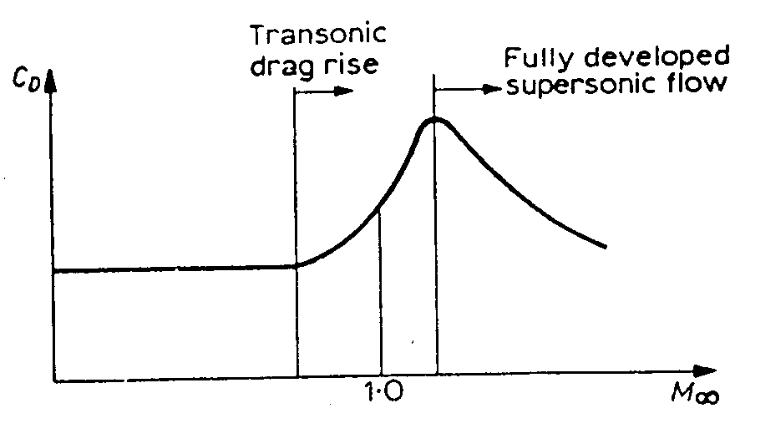
\includegraphics[scale=0.15]{ch6/2}
	\captionof{figure}{}
	\label{fig:6.2}
	\end{minipage}
	\begin{minipage}{0.3\textwidth}
	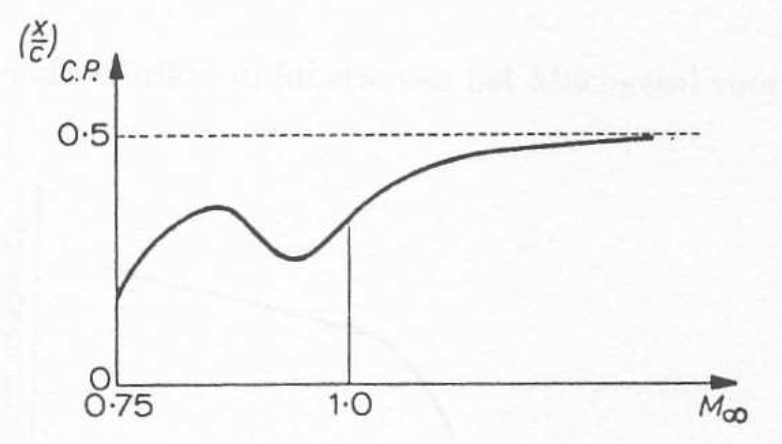
\includegraphics[scale=0.15]{ch6/3}
	\captionof{figure}{}
	\label{fig:6.3}
	\end{minipage}
	\end{center}
	
	Under transonic conditions the flow is non-stationary, the shock waves moves up and down on the wing. The pilot senses this as \textbf{buffeting} (response of the structure to aerodynamic excitation) and vibrations. This can make the plane uncontrollable or cause serious damages. The cause of the excitation is the fluctuating pressure in non-stationary conditions. Normally one flies under the buffeting margin but one can exceed it in case of sudden maneuvers for fighters for example. \\
	
	The center of pressure is also moving with $M_\infty$ (\autoref{fig:6.3}). First, it goes backward as the shock wave going backward on the suction side makes the underpressure greater. Then, it goes forward because the shock wave on the pressure side is moving faster. The latter reaches the trailing edge while the shock wave on the suction side still moves backward, making the center of pressure again move backward, tending to the 50\% chord. This makes the control of the plane more difficult. \\
	
	\wrapfig{7}{l}{5.5}{0.15}{ch6/4}{fig:6.4}
	It is this buffeting effect that imposes an upper limit to the velocity of subsonic planes. With the increase of the drag due to separation when shock waves (shock-stall) is associated a decrease of the lift. We can see that the lift temporary increases after the lower shock reaches the trailing edge. This is explained by the smaller separation when in this location. The drag divergence Mach number is 5-10\% larger than $M_{cr}$. 
	
	\ \\
	
	\begin{center}
	\begin{minipage}{0.4\textwidth}
	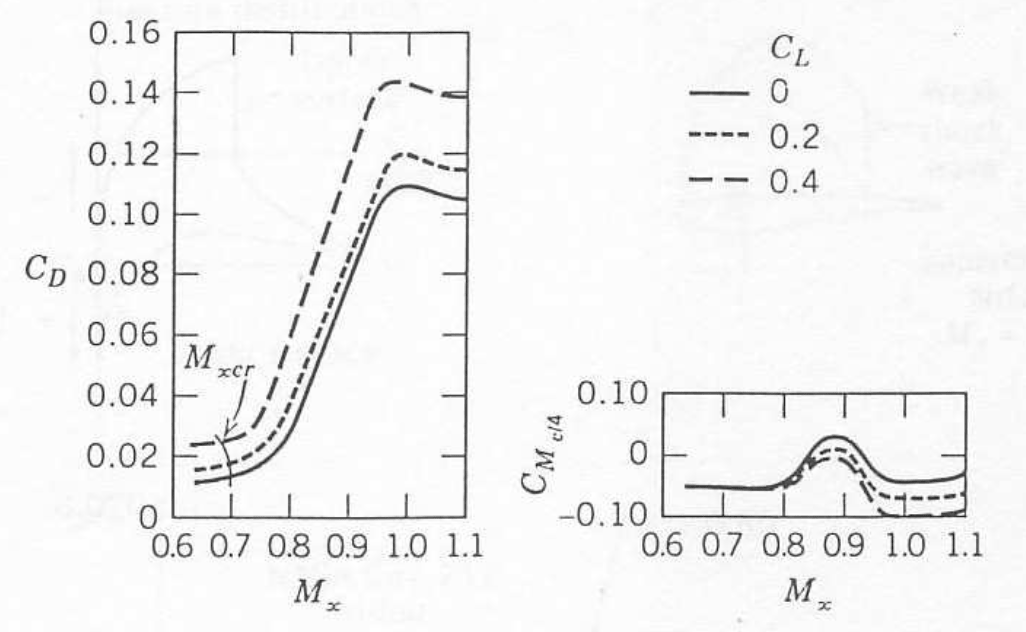
\includegraphics[scale=0.15]{ch6/5}
	\captionof{figure}{}
	\label{fig:6.5}
	\end{minipage}
	\begin{minipage}{0.4\textwidth}
	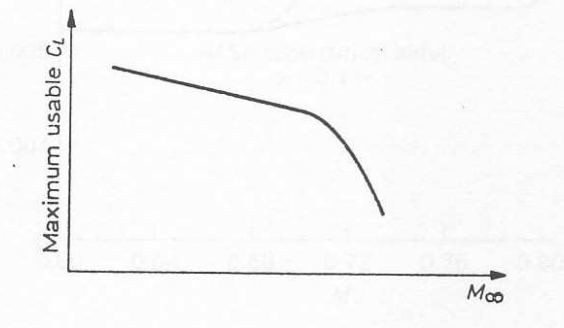
\includegraphics[scale=0.4]{ch6/6}
	\captionof{figure}{}
	\label{fig:6.6}
	\end{minipage}
	\end{center}

	On \autoref{fig:6.5} we can see the influence of increasing lift (increasing $\alpha$). We can notice that with increasing lift, the drag increases for all Mach numbers, the moment increases in the transonic region and $M_{cr}$ decreases. On \autoref{fig:6.6}, we notice that the lift coefficient strongly decreases in the transonic region due to buffering effects. 
	
\subsection{Supercritical wings}
	\wrapfig{16}{l}{9.5}{0.15}{ch6/7}{fig:6.7}
	For subsonic wings, it is thus desired to have the largest drag divergence Mach number possible. This can be achieved by using high critical Mach number wings, or increase the difference  $M_{div} -M_{cr}$. The second solution led to the supercritical wings. These have a rather flat suction side to limit the acceleration of the flow, keeping the supersonic speeds lower than other profiles and limit the strength of the shock that creates less drag. The comparison between the two type of wings is done on \autoref{fig:6.7}. We can see that the $M_{cr}$ is higher and the weaker shock wave closer to the trailing edge. 
	
	\ \\ The new shape of the suction side has a negative effect on the lift, this is compensate by an increased curvature on the pressure side near the trailing edge. On the figure we can see that the use of critical wings increases the drag divergence Mach number, that can go up to 0.99. These allows the use of thicker wings, allowing more fuel storage at lower speeds. 
	
\section{Supersonic flows}
	\subsection{The drag coefficient in a linearized supersonic flow}
	The potential equation we used in the framework of potential equation can be rewritten in the case of supersonic flow as:
	
	\begin{equation}
		(1-M_\infty^2) \hat{\phi}_{xx} + \hat{\phi}_{yy} = 0 \qquad \Rightarrow \lambda ^2 \hat{\phi} _{xx} - \hat{\phi} _{yy} = 0.
	\end{equation}
	
	The linearized potential equation corresponds to the wave equation with $\lambda ^2 = M_\infty ^2 -1 >0$. We can show that the solution of this equation is 
	
	\begin{equation}
	\hat{\phi}(x,y)= f(x-\lambda y) = \hat{\phi} _{1}(x-\lambda y) + \hat{\phi} _{2} (x+\lambda y).
	\end{equation}		
	
	Let's define 2 families of characteristic curves:
	
	\begin{equation}
	\left\{
	\begin{aligned}
	&C^+ : x-\lambda y = cst \qquad \Rightarrow y = \frac{1}{\lambda} x + cst = \frac{1}{\sqrt{M_\infty ^2 -1}} c + cst\\
	&C^+ : x+\lambda y = cst \qquad \Rightarrow y = -\frac{1}{\lambda} x + cst = -\frac{1}{\sqrt{M_\infty ^2 -1}} c + cst
	\end{aligned}
	\right.
	\end{equation}
	
	\wrapfig{8}{r}{5}{0.15}{ch6/8}{fig:6.8}
	In this way, $\hat{\phi} _1$ and $\hat{\phi} _2$ are respectively constant on $C^+$ and $C^-$. The slope is denoted $\mu _\infty ^\pm$ for $C^\pm$ such that: 
	
	\begin{equation}
	\tan \mu _\infty ^\pm = \pm \frac{1}{\sqrt{M_\infty ^2 -1}} \qquad \sin \mu _\infty ^\pm = \pm \frac{1}{M_\infty}.
	\end{equation}
	
	To find the general solution in P, let's first consider the initial data given on the y-axis: 
	
	\begin{equation}
	\hat{\phi} _1(y) = F(y)\qquad \hat{\phi}_2 (y) = G(y)
	\end{equation}
	
	Now let's construct $C^+$ and $C^-$ throw P: 
	
	\begin{equation}
	C^+ : x-\lambda y = x_A - \lambda y_A\qquad C^- : x-\lambda y = x_B + \lambda y_B.
	\end{equation}
	
	Finally, the solution in P is so given by:
	
	\begin{equation}
	\hat{ \phi} (x_p,y_p) = \hat{\phi} (x_A - \lambda y_A) + \hat{\phi} _2 (x_B + \lambda y_B) = F (x_A - \lambda y_A) + G (x_B + \lambda y_B)
	\end{equation}

	\wrapfig{8}{l}{5}{0.1}{ch6/17}{fig:6.17}
	Now let's define the initial conditions at $x=0$ for small $\alpha$ for a thin profile:
	
	\begin{equation}
	F(y) = K_1 = cst \qquad G(y) = K_2 = cst \qquad \Rightarrow \hat{\phi} = cst
	\end{equation}
	
	since the incoming flow is uniform. On the pressure side, we have $\hat{\phi} _1(x-\lambda y) = K_1$ which gives in the solution: 
	
	\begin{equation}
	\hat{\phi}(q) = K_1 + \hat{\phi}_2 (q) \qquad \rightarrow \hat{\phi}_x = \frac{d\hat{\phi}_2}{dq} = \hat{u} ^- \quad \hat{\phi}_y = \frac{d\hat{\phi}_2}{dq}\lambda = \hat{v} ^- \qquad \Rightarrow \hat{v}_{wall} = \lambda \hat{u}_{wall}
	\end{equation}
	
	If we express the tangent as $\tan \theta_w \approx \theta_w = \frac{\hat{v}^-_w}{\hat{u}^-+V_\infty} \approx \frac{\hat{v}^-_w}{V_\infty}$,
	We can get by replacing the last results in the previous pressure coefficient equation for small perturbations:
	
		
	\begin{center}
	\theor{
	\textbf{Law of Ackeret}
	\begin{equation}
	C_p ^- = -\frac{2\hat{u}^-_w}{V_\infty} = -\frac{2\theta_w^-}{\sqrt{M^2_\infty - 1}}.
	\end{equation}
	}
	\end{center}
	
	The same reasoning can be done for the suction side where we'll get:
	
	\begin{equation}
	\hat{\phi} _x = \frac{d\hat{\phi}_1}{dq} = \hat{u}^+_w \qquad \hat{\phi} _x = \frac{d\hat{\phi}_1}{dq}(-\lambda) = \hat{v}^+_w = -\lambda \hat{u}^+_w\qquad \Rightarrow C_p^+ = \frac{2\theta_w^+}{\sqrt{M^2_\infty - 1}}.
	\end{equation}
	
	\subsubsection{Application to a flat plate}
	\wrapfig{8}{l}{7.5}{0.1}{ch6/18}{fig:6.18}
	Consider the thin profile define by functions $y^+(x)$ and $y^-(x)$ with angles defines as:
	
	\begin{equation}
	\begin{aligned}
	&\epsilon = \frac{dy}{dx} <0 \qquad \theta = \frac{\hat{v}}{\hat{u} +V_\infty} <0 \\
	 \Rightarrow &\theta = \epsilon - \alpha = \frac{dy}{dx} - \alpha
	\end{aligned}
	\end{equation}
	
	as $\alpha > 0$. We can then apply the last formula: 
	
	\begin{equation}
	C_p^+ = \frac{2\theta_w^+}{\sqrt{M^2_\infty - 1}} = \frac{2\left( \frac{dy^+}{dx} -\alpha \right)}{\sqrt{M^2_\infty - 1}} \qquad C_p^- = -\frac{2\theta_w^-}{\sqrt{M^2_\infty - 1}} = \frac{2\left( \alpha -\frac{dy^-}{dx}\right)}{\sqrt{M^2_\infty - 1}}.
	\end{equation}
	
	We are now interested in computing the normal and tangential force applied on the wing, for a counter-clock contour: 
	
	\begin{equation}
	C_N = \int _0 ^1 C_p ^- \, \frac{dx}{c} + \int _1 ^0 C_p ^+ \, \frac{dx}{c} = \frac{4\alpha }{\sqrt{M_\infty ^2-1}}
	\end{equation}
	
	where we replace the $C_p$'s by their definition and we neglect $\frac{dy}{dx}$ terms. For the drag we have the same procedure but by neglecting this time $\alpha$:
	
	\begin{equation}
	\begin{aligned}
	&C_\Gamma = -\int _0 ^1 C_p ^- \, \frac{dy}{c} - \int _1 ^0 C_p ^+ \, \frac{dy}{c} = \frac{2}{\sqrt{M_\infty ^2-1}} \left[ \int _0^1 \left(\frac{dy^-}{dx} \right)^2 \frac{dx}{c} + \int _0^1 \left(\frac{dy^+}{dx} \right)^2 \frac{dx}{c} \right]\\
	\Rightarrow &C_\Gamma =  \frac{2}{\sqrt{M_\infty ^2-1}} [I^- + I^+]
	\end{aligned}
	\end{equation}
	
	To compute the lift and drag coefficient we only have to make the projections, and in case of flat plate $\frac{dy}{dx} = 0 = I^\pm$: 
	
	\begin{equation}
	\begin{aligned}
	&C_l = -C_\Gamma \sin \alpha + C_N \cos \alpha \approx -\alpha C_\Gamma  + C_N \qquad C_d = C_\Gamma  + \alpha C_N\\
	\Rightarrow &C_l = \frac{4\alpha}{\sqrt{M_\infty ^2 -1}} \qquad C_d = \frac{4\alpha}{\sqrt{M_\infty ^2 -1}}.
		\end{aligned}
	\end{equation}
	
	Remind that the drag is the \textbf{wave drag}. 
	
\subsubsection{Application to a double wedge}
	\wrapfig{8}{r}{6.5}{0.1}{ch6/19}{fig:6.19}
	If we apply the Ackeret law to this profile we have:
	
	\begin{equation}
	\begin{aligned}
	&C_{p1} = \frac{2(\delta - \alpha)}{\sqrt{M_\infty^2 -1}} \qquad C_{p2} = \frac{2(\delta + \alpha)}{\sqrt{M_\infty^2 -1}} \\
	&C_{p3} = \frac{-2(\delta + \alpha)}{\sqrt{M_\infty^2 -1}} \qquad C_{p4} = \frac{-2(\delta - \alpha)}{\sqrt{M_\infty^2 -1}}
	\end{aligned}
	\end{equation}
	
	We can compute the lift and drag coefficients by integrating over the surface:
	
	\begin{equation}
	\begin{aligned}
	&\vec{F} = -\oint p\, d\vec{S} = -\oint (p-p_\infty)\, d\vec{S} = -\frac{1}{2} \rho _\infty V_\infty ^2 \oint C_p\, d\vec{S}\\
	\Rightarrow &\vec{F}_1 = -\frac{1}{2} \rho _\infty V_\infty ^2 C_{p1} \frac{c}{2} \vec{n}_1
	\end{aligned}
	\end{equation}
	
	If we make the force non dimensional: 
	\begin{equation}
	\vec{C}_1 = \frac{\vec{F}_1}{\frac{1}{2}\rho _\infty V_\infty ^2 c} = -\frac{C_{p1}}{2} \vec{n}_1 \qquad \Rightarrow \vec{C}_i = -\frac{C_{pi}}{2} \vec{n}_i
	\end{equation}
	
	If we look to the normal and tangent forces we find: 
	
	\begin{equation}
	\begin{aligned}
	C_y = \vec{C}_i .\vec{1}_y = \left(-\frac{C_{p1}}{2} + \frac{C_{p2}}{2} -\frac{C_{p3}}{2} +\frac{C_{p4}}{2} \right) \cos \delta= \frac{4\alpha }{\sqrt{M_\infty ^2 -1}} \cos \delta \approx \frac{4\alpha }{\sqrt{M_\infty ^2 -1}}\\
	C_x = \vec{C}_i .\vec{1}_x = \left(\frac{C_{p1}}{2} + \frac{C_{p2}}{2} -\frac{C_{p3}}{2} -\frac{C_{p4}}{2} \right) \sin \delta = \frac{4\delta }{\sqrt{M_\infty ^2 -1}} \sin \delta \approx \frac{4\delta ^2}{\sqrt{M_\infty ^2 -1}}
	\end{aligned}
	\end{equation}
	
	Then we make the same projection as previously: 
	
	\begin{equation}
	c_l \approx C_y - \alpha C_x = \frac{4\alpha }{\sqrt{M_\infty ^2 -1}} - \frac{4\delta ^2\alpha }{\sqrt{M_\infty ^2 -1}}  \approx \frac{4\alpha }{\sqrt{M_\infty ^2 -1}} 
	\end{equation}
	
	We find thus the same lift coefficient as the flat plate. Let's see the drag: 
	
	\begin{equation}
	c_d = C_x + \alpha C_y = \frac{4\alpha }{\sqrt{M_\infty ^2 -1}} + \frac{4\delta}{\sqrt{M_\infty ^2 -1}},
	\end{equation}
	
	\wrapfig{11}{l}{3}{0.3}{ch6/20}{fig:6.20}
	where the first term is \textbf{incidence wave drag} (result of lift), the same as the flat plate and the second term the \textbf{thickness wave drag} (result of volume) corresponding to the drag of the wedge at 0 degrees and angle of attack. The following empirical formula can be used for both drag on wing and on \textbf{complete plane}: 
	
	\begin{equation}
	C_{Dw} = k_0 \frac{128}{\pi} \frac{V^2}{Sl^4} + k_1 \frac{1}{2\pi} \frac{S}{l^2}\lambda ^2 C_L^2
	\end{equation}
	
	where $k_0$ and $k_1$ are constant of order 1 depending on the geometry and l the average length as represented on the figure. 
	
\subsection{Supersonic wings}
	The flow properties are different from the subsonic case, as they are mainly given by shocks and expansions. Straight lines and sharp corners are as good as curved surfaces. Thus a flat plate is already the optimum theoretically, but there are structural constraints and fuel storage problems. \\
	
	Camber is thus not appropriate for the supersonic case, as the zero lift angle of attack is positive (lift negative when $\alpha = 0$). The camber reduces the lift in all incidences when supersonic. Consequently, we mainly use \textbf{symmetrical wings}. 
	
	\wrapfig{8}{l}{6.5}{0.1}{ch6/21}{fig:6.21}
	A way to realize the symmetrical wing is the so-called \textbf{double wedge} wing. The situation is at $\alpha = 0\degres$ and we can see that the pressure distribution is symmetrical wrt horizontal axis but not wrt to the vertical one, meaning 0 lift but presence of drag. The paradox of d'Alembert is no longer applied in supersonic (in non-viscous flows the pressure distribution is symmetrical wrt both axis). The drag arising because of shocks and their expansion is called \textbf{wave drag}. When $\alpha \neq 0\degres$ a lift arises, is comparable to the flat plate one but the drag is larger. 
	
	\ \\
	
	\wrapfig{7}{r}{5.5}{0.18}{ch6/22}{fig:6.22}
	Another useful profile is the \textbf{biconvex profile}. Here both sides are circle arcs of same radius. The Prandtl-Meyer expansion of the double wedge is replaced by a range of \textbf{Mach waves} (expansion waves, ch8). The leading edge shock is bent, we have more drag than the double wedge for the same t/c ratio and approximately the same lift. The leading edge angle is larger, the Mach number must be higher before the shock to be attached to the LE. 
	
	\ \\ This profile offers structural advantages and more fuel storage. In conclusion, in supersonic flight, we'd better have sharp leading edge to limit the shock drag, but this is not good for subsonic flight, take-off and landing as the stalling speed will be too low and the lift too. 